\documentclass[11pt]{beamer}

\usepackage[utf8]{inputenc}
\usepackage[T1]{fontenc}
\usepackage{amsmath}
\usepackage{amsfonts}
\usepackage{amssymb}
\usepackage{graphicx}
\usepackage{listings}

\usepackage{color}

\definecolor{codegreen}{rgb}{0,0.6,0}
\definecolor{codegray}{rgb}{0.5,0.5,0.5}
\definecolor{codepurple}{rgb}{0.58,0,0.82}
\definecolor{backcolour}{rgb}{0.95,0.95,0.92}

\lstdefinestyle{mystyle}{
	backgroundcolor=\color{backcolour},   
	commentstyle=\color{codegreen},
	keywordstyle=\color{magenta},
	numberstyle=\tiny\color{codegray},
	stringstyle=\color{codepurple},
	basicstyle=\tiny,
	breakatwhitespace=false,         
	breaklines=true,                 
	captionpos=b,                    
	keepspaces=true,                 
	numbers=left,                    
	numbersep=5pt,                  
	showspaces=false,                
	showstringspaces=false,
	showtabs=false,                  
	tabsize=2
}

\lstset{style=mystyle}

\usetheme{default}

\begin{document}
	\author{Musa Baloyi}
	\title{The Python Unittest Framework}
	%\subtitle{}
	%\logo{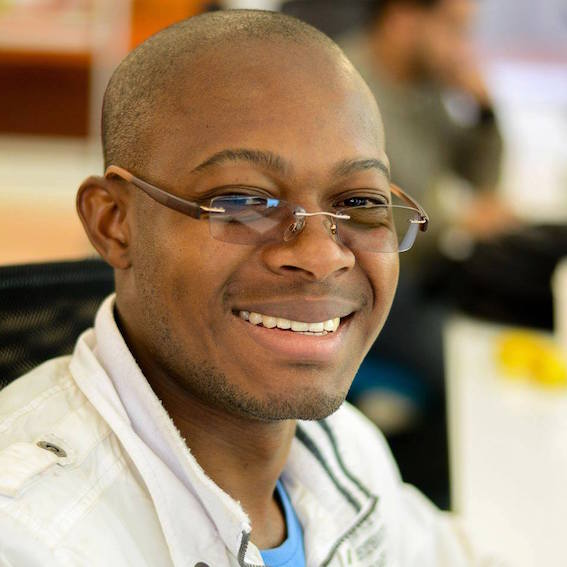
\includegraphics[height=1cm,width=2cm]{logo}}
	\titlegraphic{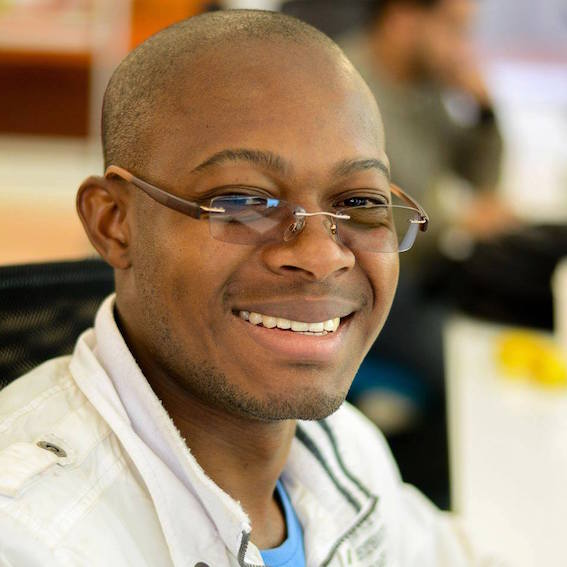
\includegraphics[width=\textwidth,height=.5\textheight]{logo}}
	%\institute{}
	%\date{}
	%\subject{}
	%\setbeamercovered{transparent}
	%\setbeamertemplate{navigation symbols}{}
	\begin{frame}[plain]
	\maketitle
\end{frame}

\begin{frame}
\frametitle{Table of contents}
\begin{enumerate}
	\item History of automated testing
	\item Components of xUnit tests
	\item Unittest
	\item References
	\item Assert statements
	\item py.test vs unittest side by side
\end{enumerate}
\end{frame}

\begin{frame}
\frametitle{The origins of automated testing}
\begin{itemize}
	\item Kent Beck designed and wrote SUnit for Smalltalk.
	\item Automated testing became a thing when Kent Beck and Erich Gamma introduced JUnit for Java.
	\item Eventually, it was ported to almost every programming language.
	\item Now most of the programming languages come pre-packaged with at least one xUnit-style test automation library.
	\item xUnit is the collective name for several unit testing frameworks for various languages.
	\item All the xUnit-style unit testing frameworks more or less derive their functionality, structure, and coding style from SUnit.
\end{itemize}
\end{frame}

\begin{frame}
\frametitle{The history of automated testing in Python}
\begin{itemize}
	\item A Python version, originally dubbed PyUnit, was created in 1999 and added to Python's standard set of libraries later in 2001.
	\item PyUnit became part of the Python Standard library from version 2.5 onward.
	\item PyUnit was the Python port from JUnit.
	\item The PyUnit library is available for both major versions of Python, 2.7 and 3.x. 
	\item unittest came to life as a third-party module PyUnit.
	\item Since then, the Python community has referred to it as unittest, the name of the library imported into the test code.
	\item Unittest is the batteries-included test automation library of Python, which requires no extra installation steps.
\end{itemize}
\end{frame}

\begin{frame}
\frametitle{Other testing frameworks in Python}
\begin{itemize}
	\item Many programming languages like Python and Java have more than one xUnit-style framework.
	\item Java has TestNG in addition to JUnit. Python has nose, pytest, and Nose2 apart from unittest.
	\item docstring and doctest and their use in writing simple, static, yet elegant test cases for Python 3 programs.
	\item Due to the lack of features like API, configurable tests, and test fixtures, doctest enjoys very limited popularity.
\end{itemize}
\end{frame}

\begin{frame}
\frametitle{Major components of the architecture of xUnit-style test automation libraries:}
\begin{enumerate}
	\item Test case class
	\item Test fixtures
	\item Assertions
	\item Test suite
	\item Test runner
	\item Test result formatter
\end{enumerate}
\end{frame}

\begin{frame}
\frametitle{Entry point of unittest is the TestCase class}
\lstinputlisting[language=Python]{../test/test_module01.py}
\begin{itemize}
	\item python3 test\_module01.py
\end{itemize}
\end{frame}

\begin{frame}
\frametitle{Order of execution of the test methods}
\lstinputlisting[language=Python]{../test/test_module02.py}
\begin{itemize}
	\item python3 test\_module02.py
\end{itemize}
\end{frame}

\begin{frame}
\frametitle{Verbosity control}
\lstinputlisting[language=Python]{../test/test_module03.py}
\begin{itemize}
	\item python3 test\_module01.py -v
	\item python3 test\_module03.py
\end{itemize}
\end{frame}

\begin{frame}
\frametitle{Multiple test classes within the same test file}
\lstinputlisting[language=Python]{../test/test_module04.py}
\begin{itemize}
	\item python3 test\_module04.py
\end{itemize}
\end{frame}

\begin{frame}
\frametitle{Test fixtures}
\begin{figure}[h]
	\centering
	\includegraphics[scale=.35]{../images/test_module05.png}
\end{figure}
\begin{itemize}
	\item python3 test\_module05.py
\end{itemize}
\end{frame}

\begin{frame}
\frametitle{Running without unittest.main()}
\lstinputlisting[language=Python]{../test/test_module06.py}
\begin{itemize}
	\item python3 -m unittest test\_module06
\end{itemize}
\end{frame}

\begin{frame}
\frametitle{Controlling the granularity of test execution}
\lstinputlisting[language=Python]{../test/test_module04.py}
\begin{itemize}
	\item python3 -m unittest -v test\_module04.TestClass04
\end{itemize}
\end{frame}

\begin{frame}
\frametitle{Command line options}
\lstinputlisting[language=Python]{../test/test_module07.py}
\begin{itemize}
	\item python3 -m unittest -q test\_module07
	\item python3 -m unittest -fv test\_module07
	\item python3 -m unittest -h
\end{itemize}
\end{frame}

\begin{frame}
\frametitle{Placing the dev and test code in A SINGLE dir}
\lstinputlisting[language=Python]{../test/test_module08.py}
\begin{itemize}
	\item python3 -m unittest -v test\_module08
\end{itemize}
\end{frame}

\begin{frame}
\frametitle{Placing the dev and test code in SEPARATE dirs}
\begin{figure}[h]
	\centering
	\includegraphics[scale=.32]{../images/test_module09.png}
\end{figure}
\begin{itemize}
	\item python3 -m unittest test\_module09
\end{itemize}
\end{frame}

\begin{frame}
\frametitle{Other useful methods}
\lstinputlisting[language=Python]{../test/test_module10.py}
\begin{itemize}
	\item python3 -m unittest -v test\_module10
\end{itemize}
\end{frame}

\begin{frame}
\frametitle{Failing a test}
\lstinputlisting[language=Python]{../test/test_module11.py}
\begin{itemize}
	\item python3 -m unittest -v test\_module11
\end{itemize}
\end{frame}

\begin{frame}
\frametitle{Skipping tests}
Decorators are used for skipping tests conditionally or unconditionally:
\begin{itemize}
	\item unittest.skip(reason)
	\item unittest.skipIf(condition, reason)
	\item unittest.skipUnless(condition, reason)
	\item unittest.expectedFailure()
\end{itemize}
\end{frame}

\begin{frame}
\frametitle{Skipping tests: examples}
\lstinputlisting[language=Python]{../test/test_module12.py}
\begin{itemize}
	\item python3 -m unittest -v test\_module12
\end{itemize}
\end{frame}

\begin{frame}
\frametitle{Exceptions in the test case}
\lstinputlisting[language=Python]{../test/test_module13.py}
\begin{itemize}
	\item python3 -m unittest -v test\_module13
\end{itemize}
\end{frame}

\begin{frame}
\frametitle{assertRaises()}
\begin{figure}[h]
	\centering
	\includegraphics[scale=.35]{../images/test_module14.png}
\end{figure}
\begin{itemize}
	\item python3 test\_module14.py
\end{itemize}
\end{frame}

\begin{frame}
\frametitle{References}
\begin{enumerate}
	\item Python Unit Test Automation: Practical Techniques for Python Developers and Testers
	by Ashwin Pajankar (2017)
	\item Python Testing Cookbook by Bhaskar N. Das , Greg L. Turnquist (2018)
	\item Unit testing framework (https://docs.python.org/3/library/unittest.html)
	\item Python Testing with pytest by Brian Okken (2017)
\end{enumerate}
\end{frame}

\begin{frame}
\frametitle{Assertions in unittest}
\begin{figure}[h]
	\centering
	\includegraphics[scale=.35]{../images/assertions.png}
\end{figure}
\end{frame}

\begin{frame}
\frametitle{More assertions in unittest}
\begin{figure}[h]
	\centering
	\includegraphics[scale=.35]{../images/more_assertions.png}
\end{figure}
\end{frame}

\begin{frame}
\frametitle{Even more assertions in unittest}
\begin{figure}[h]
	\centering
	\includegraphics[scale=.35]{../images/even_more_assertions.png}
\end{figure}
\end{frame}

\begin{frame}
\frametitle{py.test vs unittest}

\tiny{
\begin{table}
		\begin{tabular}{| l | l | l |}
		\hline
		\textbf{Property} & \textbf{py.test} & \textbf{unittest}\\ 
		\hline \hline
		Installation & Easy installation with pip & Part of standard library (None required) \\
		Color coding &  Green for PASS, Red for FAILURE & No color coding (External library required) \\
		Paradigm & Functional and object-oriented & Object-oriented (OOP) only \\
		Interoperability & Can run unittest and nose tests & Lower level \\
		Test runner & py.test; -m pytest & python; -m unittest; py.test; nose \\
		Usage & Command line flag & import statement \\
		Test discovery & Through py.test & Through python -m unittest discover \\
		Verbosity & Through -v & Through -v \\
		Fixtures & xUnit and custom & xUnit (Decorators can be function calls) \\
		Granularity & Down to test method & Down to test method \\
		Assertions & Through assert & Through assert<Equality, Truth, DataType, etc> \\
		Exceptions & pytest.raises() & assertRaises() \\
		Command line & Much more extensive options & Extensive options \\
		\hline 
	\end{tabular}
\caption{Let's battle it out!!!}
\end{table}
}
\end{frame}


\end{document}